\documentclass[12pt,a4paper]{report}

\usepackage{geometry}
\geometry{a4paper, margin=2.5cm}

% space between paragraphs (has to be big since there's no indentation)
\setlength{\parskip}{\bigskipamount}

% indentation length
\setlength{\parindent}{0pt}

% setting leading (i.e., line spacing)
\usepackage{setspace}
\onehalfspacing

\usepackage{graphicx}
\usepackage[hypertexnames=false]{hyperref}
\usepackage{listings}

\usepackage{color}
\usepackage[usenames,dvipsnames,svgnames,table]{xcolor}

\hypersetup{
  pdftitle={Design of semantic mashup for extracting restaurant data by scraping},
  pdfauthor={Deepan Murugan},
  pdfkeywords={ python, semantic mashup, screen scraping },
  colorlinks=true,
  linkcolor=black,
  anchorcolor=black,
  citecolor=black,
  urlcolor=black,
}

\begin{document}

\pagenumbering{roman}

\begin{titlepage}
  \begin{center}
    \textsc{\LARGE UNIVERSITY OF WARWICK}\\
    \large Department of Computer Science\\[1.5cm]
    
    \textsc{\LARGE Design of a semantic mashup for extracting restaurant data by scraping}\\[1.5cm]
    by\\[0.4cm]
    \textsc{\Large Deepan Murugan}\\[1cm]
    \large{\emph{Supervisor}: \textsc{\Large Dr. Alexandra I. Cristea}}\\[1.5cm]
    
\includegraphics{fig/crest_fullcolour.pdf}\\[1.5cm]
    \LARGE September 2012
    
  \end{center}
\end{titlepage}

\cleardoublepage
\phantomsection
\addcontentsline{toc}{chapter}{Table of Contents}
\renewcommand{\contentsname}{Table of Contents}

\tableofcontents

\setcounter{secnumdepth}{-3}

\cleardoublepage
\phantomsection
\addcontentsline{toc}{chapter}{\listfigurename}
\listoffigures

\chapter[Acknowledgements]{\centering Acknowledgements}

First and foremost, I would like to thank my supervisor, Dr. Alexandra I. Cristea,
for her immense assistance and feedback during the project thesis.

I am also grateful to my classmates and the PhD students of the department,
who provided me with insights,ideas and help during my research and programming.

Finally, I am thankful for the Python community for providing an excellent language 
and easy to use libraries, which made my life easier and my code simpler and efficient.
\chapter{Abstract}

Mashups represent a new era of interactive web applications, which are quickly gaining popularity. They combine data and services to provide new functionality with emphasis on user interactivity. Mashups also harness the latest Web 2.0 tools to provide a more collaborative user experience. This thesis explores the meeting point of Web 2.0 and the Semantic Web, by focusing specifically on the emerging technologies of mashups, but also exploring semantically relevant annotations of the retrieved results, and then creating an application to illustrate the lessons learnt. We present a semantic mashup that can provide information on suitable restaurants based on a range of collated parameters. Our mashup involves integrating data from from two sources and provide categorized results based on the extracted data. We illustrate the effectiveness of the approach and the implementation with a case study and provide a basis for a more customizable functionality.

\textbf{Keywords:} python, semantic mashup, screen scraping, Web 2.0


\setcounter{secnumdepth}{2}

\pagenumbering{arabic}

\chapter{Introduction}
\section{Motivation}
    The World Wide Web is the main source of information nowadays. Today, there exists a great demand for getting the exact information, which is embedded across millions of web pages spread across the internet \cite{1}. Here, mashup applications come in handy.
     
A Mashup is a web page or application that consolidates data and functionality from one or more different sources and provides a new kind of service \cite{2}. Its main features include gathering data, processing it and providing visually enhanced information. This field is gaining increased attention and is extensively studied.

There are several advantages in using mashup applications rather than simple web apps. For instance, mashups can organize and present the data faster than accessing it manually from different web sites. They can also provide a user friendly interface with easy data manipulation as the prime purpose for the users.

Mashups range from simply integrating data from different sources, to providing new services. Mashups harness the power of Web 2.0 applications in order to provide a more diverse user-centric experience. Semantic mashups are our focus of study due to the fact that the extracted data can be semantically annotated to make it more valuable and informative since their primary goal is to add meaning to the data \cite{1}.

Mashups can be used in various kinds of applications. For example, the first popular mashup website called housingmaps.com gathered available housing rent data from real estate websites and mapped those to locations using Google maps, so that the user is able to check houses available for rent visually. Several features, like real-time updates, were provided to ensure the correctness of data changes. Another common Web 2.0 feature is sharing the new found information via Facebook or twitter, which acts as a user contributed information.

At present, there are many kinds of mashups applications available on the internet. They all have different design approaches. Some are designed solely using predefined tools like the widgets of Yahoo pipes \cite{25} or the Microsoft Popfly \cite{26}. But mainly, mashups are designed by developers with programming expertise and these designed mashups offer better functionality than the ones created using widgets. Most mashups have different ways of gathering data and provide a new service by allowing the user to process that data to provide meaningful information.

Our motivation is to design a semantic mashup with the use of a focused web scraper. This can scrape relevant data of a topic of interest and append them with semantic annotations to display information with meaningful value. Web crawlers and web scrapers are mainly used by search engines for searching and displaying hyperlinks to the relevant web pages. Using a focused scraper for a particular website and scraping bits of data from it can be a useful and unique approach for data gathering.

\section{Scope of project}
Mashups relate to a vast area of research and our scope is limited to the web scraping techniques involved and how they can help in assisting the semantic mashup application. The main task is to extract semantic data from different web pages and collate them in an organized way.

In answering the need for an easier access to the required data, the first aim of this project is to design and implement a focused scraper for multiple websites. It will be able to focus on specific topics of interest, which in our case are restaurants of different cuisines. The scraper should be able to scrape the necessary web pages of a particular restaurant and gather all the data into a single place.

Normally, all web pages are described using HTML markup tags. Its quite a challenge to deal with structured and unstructured web pages spanning the internet. Here is where Python’s external libraries are useful. Several libraries like beautifulsoup \cite{5} and mechanize \cite{6} have been defined and are used in this thesis. These have specific functions that include parsing standard HTML markup tags and are suitable to accomplish our tasks and hence the Python programming language was used.

Once we have the extracted data, the next step in the project is to present the data semantically i.e. add meaning to the data to make it more informative. This core task is defined in \cite{1} which adds metadata to the information and increases its value. Suppose for instance, for a restaurant, the information of interest are its reviews, statistics, health ratings. In our case, these are collated from multiple different sources. All this information can be collated into a specific portfolio for that restaurant and users can judge its value and can decide whether to visit the restaurant or not. Predefined semantic annotations can be set such that when new restaurants data is available, they can be easily appended and categorized.

This semantic mashup can then be customizable, such that new restaurant details can be added at ease with predefined annotations. In particular, this project focusses on the different ways of extracting the data from the web sources and providing the various annotations for the data for clustering and grouping it in semantically relevant ways.

\section{Objectives}
The objectives of the dissertation are as follows:

\begin{enumerate}
\item To design a focused scraper that can extract data from web pages of varying formats.
\item To provide semantic markup and organize the extracted data in order to make it more meaningful, thus adding semantic data.
\end{enumerate}

Experimental results will be analyzed and discussed with a suitable case study.

\section{Overview of dissertation}
The rest of the dissertation is structured as follows:

Chapter 2 provides a literature review which is an overview of related work in the area of mashups and the challenges being addressed. This chapter provides further details regarding the types, design approaches and the use of web scrapers and crawlers.

Chapter 3 describes the methodology used. We illustrate the design process of the focused scraper for scraping restaurant websites. Then we describe the approaches for web scraping and details on the working of the scraping program.

Chapter 4 details the implementation of this crawler and execution of it using various queries on the specified web pages. The approach is tested by exploring the effectiveness of the program and if it is providing the appropriate results. Finally, further evaluations are conducted via a user survey.

In chapter 5, we report an analysis of the obtained results and the limitations and difficulties encountered. We also provide a discussion of the results and compare them via a suitable case study.

The last chapter concludes the thesis with directions for potential future work and a summary of the work done.

\chapter{Literature review}
This chapter aims to review the various types of mashups. It provides details that were researched by reading the academic papers and cites work that influenced the developing of our semantic mashup. In particular, general mashup architectures are studied, and the design process is thoroughly researched. Our focus is mainly on semantic mashups. Thereafter, a study of the problems and challenges encountered in designing such mashups are studied and analyzed.

\section{Research on web Mashups}
Mashups are distinguished based on their data and the services they provide. According to the programmable web \cite{23}, a huge number of mashups exist. Due to the abundance of data and services available, even end users are able to create simple mashups, based on predefined templates. A typical architecture of a mashup is usually divided in three layers \cite{4}:
\begin{enumerate}
\item \textbf{Content source:} These sources will have the data embedded in their web pages. Normally, some web sites provide APIs for their data systems which can be used for showing the data. Although some content providers may not have an implementable API yet, there are ways to get around this and employ techniques of screen scraping to gather data of interest. Content sources for our mashup are the web pages of interest from different web sites that contain the data on restaurants.
\item \textbf{Mashup UI:} This is the user interface for the semantic mashup application. This represents the presentation layer and user interfaces of mashups can be customized according to various needs. A proper design of the user interface can determine whether an interactive user experience can be provided. For instance, the user inserts a query with the UI and the query is processed and the results obtained are presented in an aesthetically pleasing way potentially based on user preferences. Client-side applications are normally used but server-side solutions exist as well.
\item \textbf{Platform:} This is often disputed as a third layer. \cite{4} specifies this as the client web browser where the mashup UI is running so the web browser acts as the \textsl {de facto} standard platform.
\end{enumerate}

\subsection{Mashup creation}
Some mashups follow a particular generation process which entails a set of guidelines. We specify an overview of a general process to create a semantic mashup pertaining to data aggregation. Our mashup is a data aggregation type since it involves a heavy use of data. The data retrieved is first cleaned and processed for suitable data modeling. Then the modeled data is gathered and processed with suitable parameters and then published to provide the mashup outcome. The original data from the source is never altered, although indirect access is available within the source’s web pages.

\subsection{Mashup examples}
Before the dawn of Web 2.0, most mashups were simple such that they utilized non Web 2.0 applications such as Google maps and we had to depend on existing content available on the net.But the advent of Web 2.0 changed all that. From content consumers, we became content providers and it was fairly easy to collaborate with other interested users and create mashups using Web 2.0 and other tools. The arrival of Web 2.0 paved the way for generating metadata about users and content, as well as changed the way developers deal with data. All this metadata is widely used in recommender systems and for generating user profiles, in order to make decisions about users’ interests.

Most examples employ the use of Google maps, since the Google maps API is freely available. Location based information is the main purpose for using Google maps. Recently, Web 2.0 applications such as YouTube, Facebook are also shown profound interest in the mashup development community. The use of social and professional networks can help in collaboration among users and sharing of mashup processed information.


\section{Mashup types}
Mashups are created based on different requirements. There are many types and categorizations of mashups. The most common types are the ones utilizing Google maps. Being called mapping mashups \cite{4}, these mashups use the Google maps API in providing location data that can be presented visually on the map.

Personalized mashups are taking center stage due to the advent of photo and video websites like Flickr and YouTube. These kinds of mashups involve user generated content of photos and videos with a host of features provided by the websites and their APIs. Some examples can include creating a collage of various photos with some background music of a suitable genre and using profile data of social networks for a more personalized feel \cite{4}. These mashups are more focused with the user context in mind. News websites can also be taken as an example of personalized mashup in terms of providing the users with recommended articles relevant to their genre of interest.

Some other useful mashups, like search and shopping mashups have widespread use due to their ability to collate price data from many shopping sites. Amazon and eBay have opened up access to their data via APIs, which means they can also be collated. For instance, there was an interesting mashup \cite{10}, which collated the current prices of a chosen book from various shopping websites. It displayed the rates of the book and helped users in deciding to purchase the book from the site with the lowest rate or based on other information. This would have used the APIs of the respective shopping websites in order to scrape their relevant data and make a decision after using it.

\begin{figure}[!h]
  \centering
  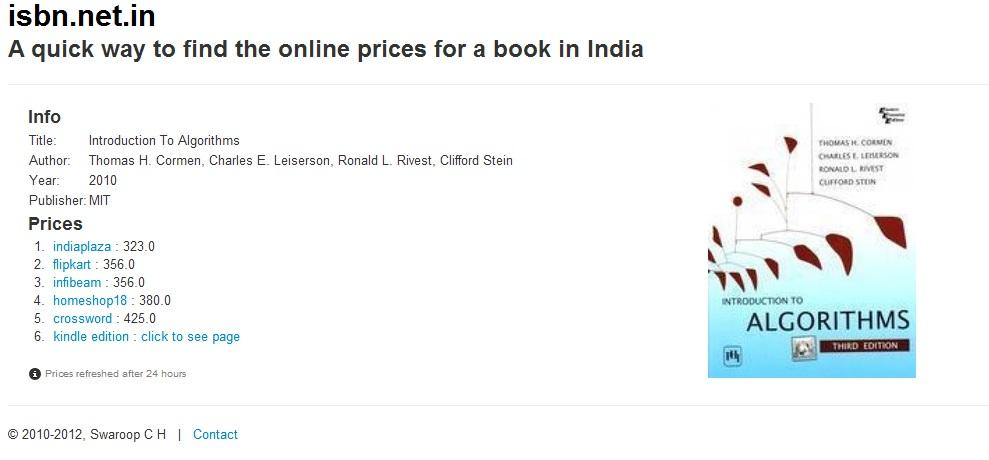
\includegraphics[width=16cm]{fig/book_price.jpg}
  \caption[Example of price comparasison mashup]
  { a mashup for finding online price for a book from various shopping sites. The results of a query of an ISBN number are displayed above.}
\end{figure}
\clearpage

Some mashups are categorized in terms of data visualization for instance where the data is simply displayed in an appealing way using various visualization techniques. Facebook’s timeline feature can  serve as an example of a data visualization mashup since it just takes the data and presents it in a timestamp based format akin to the data entries in chronological order. There are some image search engines which can display items visually in lists, graphs etc. and use some item-related attributes such as dates of last uploaded, prices, items of rank based order \cite{1}.

We focus mainly on data aggregating mashups since we are striving to design our semantic mashup by extracting data from multiple sources and finding ways to collate it by adding semantics. More emphasis is placed on the extraction strategies and we shall look into them in the later part of this chapter.

\section{Approaches to mashup development}
Here, we discuss the various tools and programming methodologies used in creating the mashups that we see today. They mostly involve widget tools, web technologies etc.

\subsection{Widget based tools}
There are a variety of software tools online that boast ease of use, helpful for non-programmers and rapid development of dynamically enhanced mashups. The research paper Mash maker: Mashups for the masses described it as an interactive tool which can be used to edit, manipulate, query and visualize live semi-structured data \cite{13}. The main advantage of using mashup making tools is that no prior experience of programming is needed as non-experts can use it effectively. However, the problems associated with using these kind of tools is that the user will have many restrictions and in some cases, the data will have to be live and visualizations and manipulations can be done only to some extent.

Some of the famous tools like Yahoo pipes, Microsoft Popfly and Dapper from \cite{14} claim that users with no programming background can easily use these tools to develop mashups on their own. Microsoft Popfly is deprecated as of now. Yahoo pipes relies heavily on RSS feeds and uses a widget approach where users can choose existing widgets that perform specific operations and they can be customized \cite{14}. Some of the problems associated in using these are that it will be difficult to keep track of all the widgets involved and since the widgets are pre designed for specific purposes, they may not support any new purposes. Even though mashups are designed using these tools, the created mashups are restricted to only some kind of functionality that can be made with respect to the preformatted widgets used in these tools.

There exist some tools that can be used for specific purposes such as data extraction. Mashup enablers help in extracting content from different web sites without any need for novice knowledge. These tools can be used effectively for web sites whose layouts get changed constantly and the main advantage is that they provide access to the unstructured content of web pages which would otherwise have been difficult to achieve as specified in \cite{15}.

However, these tools will not be effective, as they can only extract parts of website that are easily recognizable via the web pages source code. They will benefit in gathering information for mashups but the thesis project involves case studies of extracting data from unstructured web pages, the queries involved are being user generated, and thus the outcomes can get changed based on different user queries.

\subsection{ Web technologies}
Some of the research papers explained about the most important web technologies that can be used in developing mashups. A widely used tool is Asynchronous JavaScript over XML (AJAX) which is appropriate for developing mashup applications due to its real time syndication. There are several advantages using specific tools in \cite{16}, for instance they can also be useful for data to be integrated across web feeds, various sites etc. To satisfy the thesis objectives, a Python web framework was used to support dynamic display, and processing of asynchronous data retrieval XML http requests.

JavaScript is very useful for designing mashups since most of the APIs are coded in JavaScript. For instance, Google search API is written in JavaScript. It’s also the scripting language of the web and is useful for adding dynamic functionalities in web pages.

For selecting a suitable web programming language, we chose Python for its simplicity and ease of use. It is soon becoming the \textsl{de facto} programming language for the web. With respect to our goals in the project regarding data extraction, \cite{5} and \cite{6} are popular Python libraries, which make it easier to extract data from HTML and XML files. The documentation has several examples which were researched akin to our project goals and were well correlated. Programming the focused scraper also gives us more control over our mashup design and hence,-  a versatile application can be built catering to the needs of the user specific queries.

\subsection{APIs and web services}
As already said, the most widely used API in mashups is Google maps. This can be found in a wide variety of mashups where it requires the location to be displayed. Amazon has also made its API freely and publicly accessible and, as said, can be used to display their content \cite{17}. The Google search API is another famous interface which can be implemented, such that Google search results can be displayed in the mashup and it can be programmed to provide specific results based on keyword searches.

Although the API’s have user friendly tutorials with lot of examples catering to the needs of any kind of user, its required that the user should be skilled at least in an intermediate level of a programming language, in order to use these APIs effectively. Therefore, a relatively detailed knowledge of a  programming language is required, in order to integrate these API’s into ones mashup application.

Not all of the websites will have an API, and often other techniques are required to extract the data one needs. There are also ethical and social challenges involved, if websites don’t want to share their data with other parties \cite{4}.

\subsection{Screen scraping}
Due to lack of APIs for some webpages, screen scraping is a useful technique in retrieving the information from the data sources. As the name implies, it is the process of parsing and analyzing the source code of a web page, in order to extract the semantic structure of the data. In our project context, web scraping is more appropriate, since we deal with HTML web pages, and thus it represents a useful technique in accordance to our project goals.

Despite the merits, \cite{4} specifies that there are some issues with this method. For instance, the scraping method should be modeled akin to the source code of the web page, and this could prove difficult, if different web pages are created by using different formats. Web sites often undergo changes in representing their data in order to get a different visual feel and this can hinder the scraping tool’s chances of successful extraction of data. In our project, we aim to deal with a challenge such as this and we illustrate case studies for a website with one format and a second website with a different format.


\section{Problems with mashups}
Some of the research papers referred to how mashups benefit users as well as what kind of problems did the mashup developers encounter. Most of the problems that occur were due to the reliability of the API to be used, its documentation and issues with coding the mashup \cite{8}. Even though an API exists for a web site that is to be mashed up, this doesn't guarantee ease of use of wide take-up, as there might be some problems with understanding the documentation of the API \cite{19}.

\cite{4} indicated some data integration challenges. This mainly refers to issues which can be encountered with the data involved. There might be issues with the data models and sometimes with the data itself. Due to the source models being third party, mashup developers may not be familiar with them. Some of the data may either be missing or not suitable for automation into the mashup and hence, additional preprocessing is required. This is where semantic modeling comes in as stipulated in \cite{4}.

Moreover, there are several open challenges regarding the usage of data, from social and, ethical points of view. Any data used will have to be referred back to the original source. Some content providers will have control of its data as intellectual property and will instigate a fair use policy \cite{4}. These shouldn’t be much pondered upon as long as content owners’ guidelines are met.


\section{Web scrapers vs web crawlers}

Web scraping is plausibly different from web crawling. The former denotes information retrieval from websites with emphasis on data. Web scraping mainly deals with transforming unstructured data from html pages to readable data. Web crawling usually deals with indexing the web with web pages related to some domain. Research on web scraping came to light in \cite{22}, which aimed to combine data and services from web sources with a dedicated tool. This tool can be useful in accomplishing the data extraction tasks, after which data are present individually as web output. Its emphasis is placed on data. It provides operators to take relevant data as input, process it via a data flow architecture that can add metadata. The output is provided on a spreadsheet, which is later processed by end user to add to required services (like maps, for instance) and is published as output.

\chapter{Design}
This chapter aims to introduce and discuss various aspects of the design process for the semantic mashup and the working of the focused scraper. In particular, the first section will provide some background context on website scraping. Then, the detailed design of the semantic mashup and the focused scraper program will be introduced. Then, an account is following on how the focused scraper can be managed in the mashup application.

\section{Scraping techniques}
Web scraping is the technique of automated information extraction from one or more web sites. Web scraping uses many strategies, to achieve this goal. The ones used for this thesis are described below.

\subsection{Using regular expressions}
One strategy for web scraping is that of, using regular expressions to analyze the source code of the target web page. A regular expression is a piece of string that describes the structure of a larger text. Since all web pages are made out of text, excluding images and videos, regular expressions are effective. With the help of regular expressions, bits and pieces of the page can be examined in isolation. For example, “<p>.+?</p>” will match a paragraph of text. Although regular expressions are useful, they can not be used to parse HTML fully, because HTML has too many rules and exceptions. To parse HTML fully, we need a HTML parser or a DOM parser.

\subsection{Using DOM parsing}
An HTML document once parsed, becomes a DOM object, in the browser. On a DOM object, a number of useful operations like, selecting all headings, selecting particular section, selecting a particular class of paragraph elements can be performed. There exist many libraries in Python that simulate the browser and create a DOM object. We have used Beautiful Soup 4 \cite{6}.

\subsection{Web Robot Programming}
A web robot simulates the actions of a user in a browser window. For example, if the user
\begin{enumerate}
\item Opened a browser
\item Typed www.google.com in the URL bar
\item Pressed 'Enter'
\item Entered a query “restaurants in Liverpool”
\item Pressed “Go”
\item Clicked on the first result
\end{enumerate}

The user is displayed the first result's web page. In this case, namely \\
\emph{http://www.gustorestaurants.uk.com/restaurants/gusto-liverpool}. All these actions can be simulated programatically with the help of a Web Robot, often shortened to as a bot program.

As it can easily be imagined, using a bot one can simulate many actions on a website and one can extract useful information after an interaction with it, virtually. Interactivity with the web page in question is the key feature that differentiates crawling from scraping. Python provides an excellent library, specialized for bot programming, which we have used.

\section{Content Sources}
The content sources of our mashup are the following three: \emph{restaurant-guide.com}, Google maps and \emph{ratings.food.gov.uk}. The first website provides restaurant details like cuisine, address, opening/closing timings, phone. Google maps provides us with a map pointing to the restaurant location. And finally the latter provides food hygiene ratings from the Food Standards Agency of UK.
Below the first of the sources is displayed.

\begin{figure}[!htb]
  \centering
  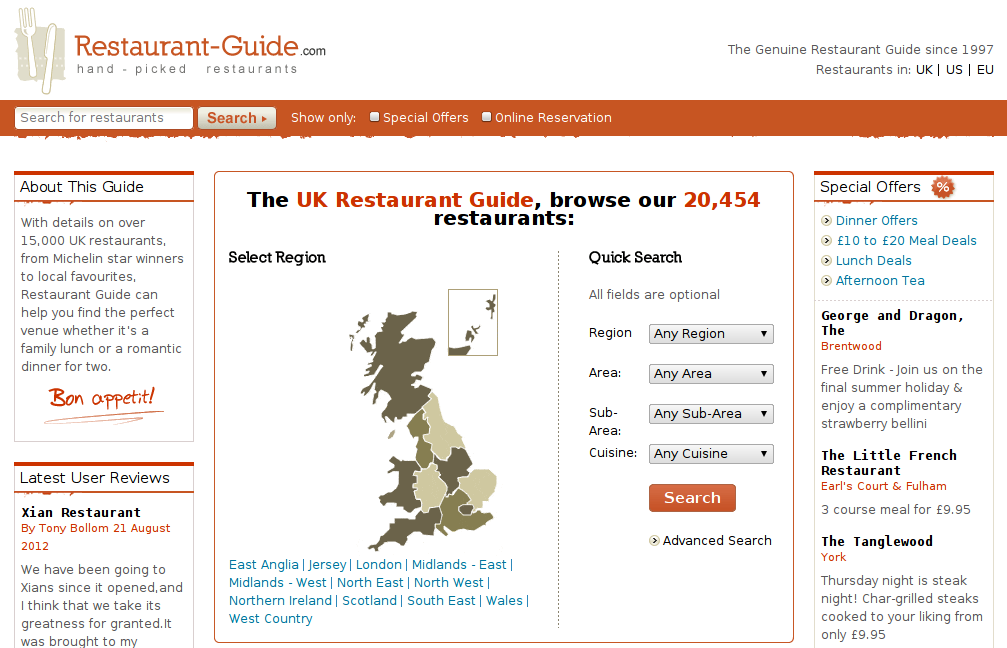
\includegraphics[width=16cm]{fig/restaurant_guide.png}
  \caption[ http://restaurant-guide.com]
  {shows our content source restaurant-guide.com}
\end{figure}

\begin{figure}[!htb]
  \centering
  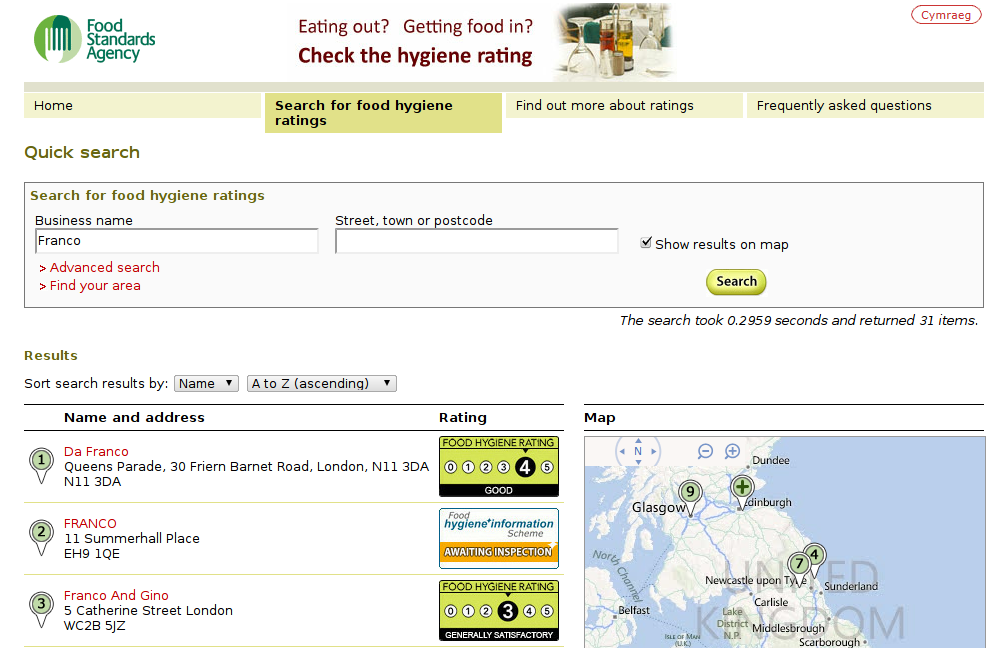
\includegraphics[width=16cm]{fig/fsa_ratings.png}
  \caption[ http://ratings.food.gov.uk]
  {shows another content source ratings.food.gov.uk}
\end{figure}


\section{Mashup User Interface}

We have given our designed application, a simple name: we call it 'RestaurantGO'. For the mashup to work, the user just has to type the cuisine name and run the search. For instance, 'Italian Coventry'. It will provide results of a list of restaurants with predefined semantic annotations.

\begin{figure}[!h]
  \centering
  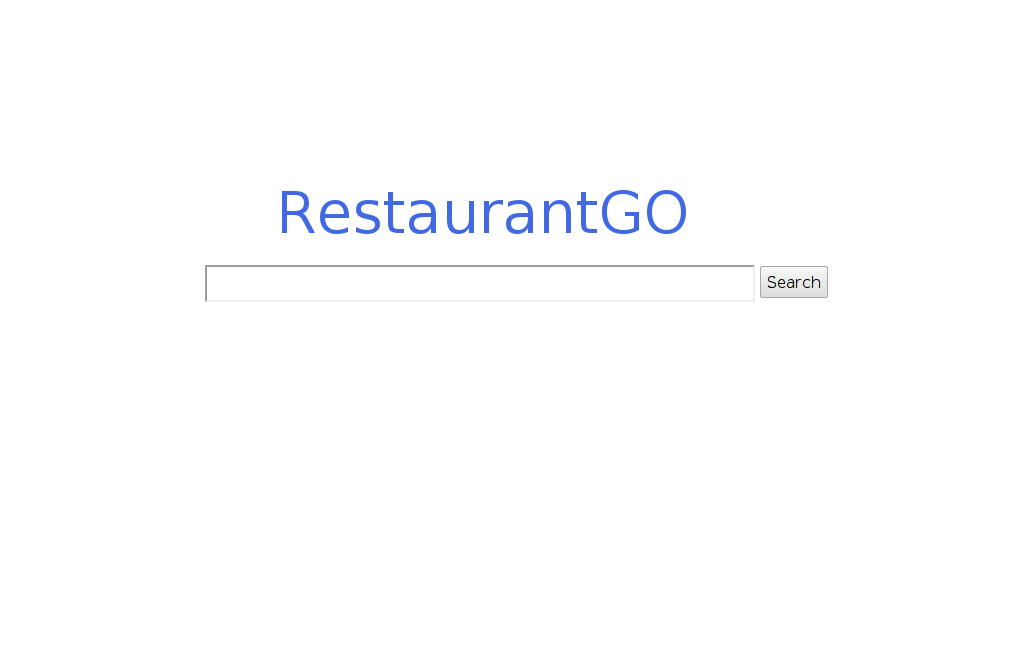
\includegraphics[width=16cm]{fig/restaurant_go.png}
  \caption[ RestaurantGo home page]
  {shows home page of our mashup RestaurantGo}
  \label{fig: 3.3}
\end{figure}

The results were obtained by scraping the source website restaurant-guide.com which searches for Italian restaurants and gathers the data for every restaurant record. These attributes for every restaurant are categorized under our custom designed columns such as address, type of cuisine, phone, opening times, lunch and dinner prices. Google maps location based information was also obtained. In the next section, we move onto the working of our mashup.

\newpage
\begin{figure}[!h]
  \centering
  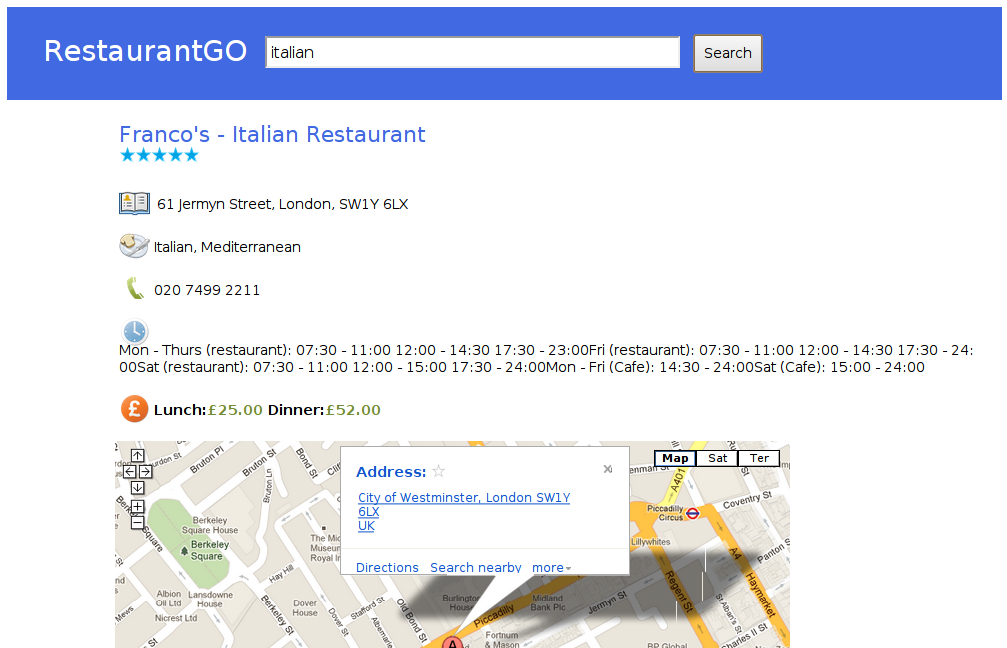
\includegraphics[width=16cm]{fig/restaurant_go_results.png}
  \caption[ RestaurantGo search results]
  {shows RestaurantGo's search results for Italian cuisine}
  \label{fig: 3.4}
\end{figure}

\section{Scraping program}
Our program involves running a local server on a client browser. In order to accomplish this, we have to install certain Python libraries. They are:
\begin{enumerate}
\item \textsl{Flask:} This is a small framework in Python which has a built-in development server \cite{24}. This was considered suitable for our project. Its methods were used to run our GET method and render custom designed html files.
\item \textsl{BeautifulSoup:} It’s a Python library useful for extracting data from HTML and XML files \cite{6}. It works along with an html parser and has many objects suited to working with html tags in scraping data.
\item \textsl{mechanize:} This is another another library useful for web programming in Python. The main feature is that we can emulate a browser and task automation \cite{5}.
\item Other standard packages \textbf{sqllite 3, re, json, urllib}, are all available in Python 2.7. \textsl{SQLite} is used for storing the results obtained. \textsl{urllib} is used for parsing the related web pages via their URLs. \textsl{json} is an object notation library for presenting results via a suitable format.
\end{enumerate}

\subsection{Architecture}
To get an overview of the application created in this research thesis, RrestaurantGo, it is important to understand the architectural principles involved in building it. RestaurantGo is first and foremost a Flask Web Application. Flask framework internally follows the REST paradigm. REST is a predominant web service design model. It utilizes the HTTP protocol verbs “GET”, “POST”, “PUT”, “DELETE” and others to build web services on top of it. Once the Flask Web Application server (HTTP Server) is started, each and every Form submitted, and the URL entered in the URL bar or clicked on the page, maps to a REST call like “GET /url”. These calls are called “routes” by the Flask framework. Each route has a handler which gets executed and serves the particular web page or a web resource. The user interacts with the web resource and produces more REST calls as a result of his actions. And in this way the user-application interaction cycle continues, till the the user reaches his goal.

\begin{figure}[!htb]
  \centering
  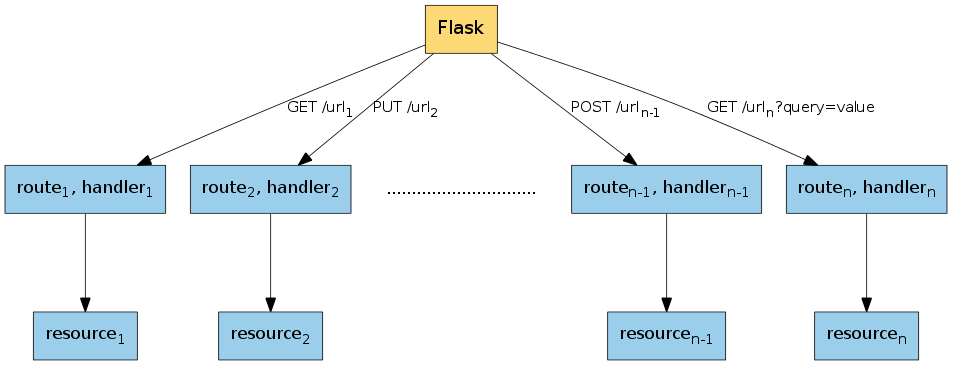
\includegraphics[width=16cm]{fig/flask.png}
  \caption[Workflow of a Flask application]
  {shows workflow of request and routes in a Flask application}
\end{figure}

The above figure shows how the Flask framework, in general serves web requests. Once the Flask HTTP server starts, it listens to various HTTP requests like “GET”, “PUT”, “POST” initiated by the user. For each request a handler gets executed which serves the results. In the context of our mashup application, see Figure ~\ref{fig: 3.6}.

\begin{figure}[!htb]
  \centering
  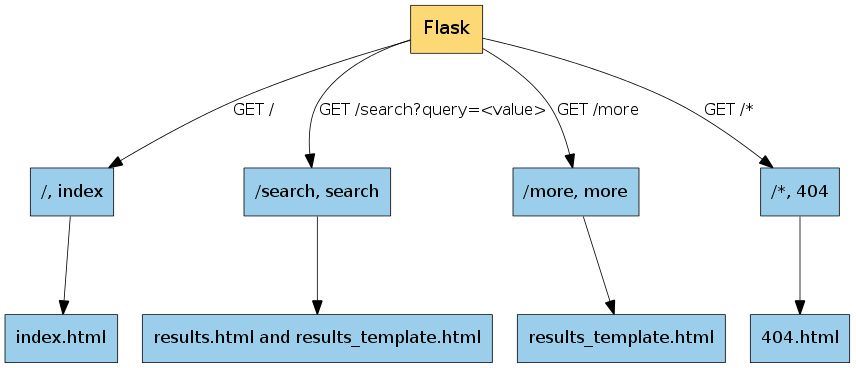
\includegraphics[width=16cm]{fig/rest.png}
  \caption[Workflow of RestaurantGo]
  {shows the REST workflow of Flask in RestaurantGo}
  \label{fig: 3.6}
\end{figure}



After starting the web server, when the user enters the url \emph{localhost:5000} in his browser, the user is immediately presented with the contents of index.html (Fig ~\ref{fig: 3.3}). This is because, “/” is considered as the route when only the url is given. Now from that page,the user can enter a query in the search form. Once the search button is clicked, the user is directed to the results.html page (Fig ~\ref{fig: 3.4}). Between the search request and the delivering of the results, the “search” handler gets executed. It is this handler that scrapes the content sources. Similarly when the user wants more results from the results page, he clicks ``More Results ...'' and this executes the more handler through the /more route, asynchronously using AJAX. The more handler returns more of the scraped results, which gets added to the already existing results by JavaScript. Finally, when the user enters a wrong URL, he is promptly showed the standard 404 Not Found web page.

The functionality of the mashup is delivered by the search and more handlers. Since both are similar in design, we will discuss the search handler below.

When the user enters a search query for “Liverpool”, the following micro-actions happen:
\begin{enumerate}
\item The browser sends a “GET  /search?query=Liverpool” to Flask
\item Flask deciphers the GET request and retrieves the corresponding route, here – “/search”
\item Flask starts the execution of the handler for “/search” route, which in this case is “search”.
\item Search handler stores “Liverpool” under the cookie name “query”. This will come in handy when the \textsl{more} handler gets executed. Because cookies are persisted across web requests, the more handler can know the query implicitly via the browser cookie.
\item The database is queried for “Liverpool”. If it is a hit, no further processing is required and one can directly jump to step 9.
\item If the Database query is a miss, then it means we have to scrape the results from the content sources. To do this a special helper class “RestaurantGuide” is called upon. The idea of using a special helper class is to isolate all the scraping logic of a content source into a separate module. Then, the search method of Restaurant Guide is called.
  
  
  
\item The scraping actions of the search method, performs the following:
  \begin{itemize}
  \item Creates a virtual browser object using mechanize.
  \item Open www.restaurant-guide.com in the virtual borswer
  \item Find the search form and submit “Liverpool” there.
  \item Wait for the result. The result is a HTML page.
  \item Pass on the result to BeatifulSoup DOM parser.
  \item Extract the restaurant data from restaurant-guide.com with the help of BeautifulSoup.
  \item Repeat the above process for ratings.food.gov.uk. Except this time, use regex for parsing.
  \item Return the extracted data to the search handler
  \end{itemize}
\item With the results in hand, the search handler now stores the results into the database for future use.
\item The results and a template “results.html” are taken and rendered to the user with the help of Flask's render\_template function. A template is a special html file. Since HTML is a declarative language, it does not support variables, if and while loops. A template consists of precisely these extra features. However, a browser cannot understand these features. Therefore a template has to be pre-processed to remove and evaluate the extra tokens. That is the job of render\_template.
  
\end{enumerate}
The flowchart of the workings of our mashup is given in the next page.

\begin{figure}[!htb]
  \centering
  \caption[Flowchart showing the working of  RestaurantGo]
  {shows the working of our Mashup -- RestaurantGo}
  \vspace{0.8cm}
  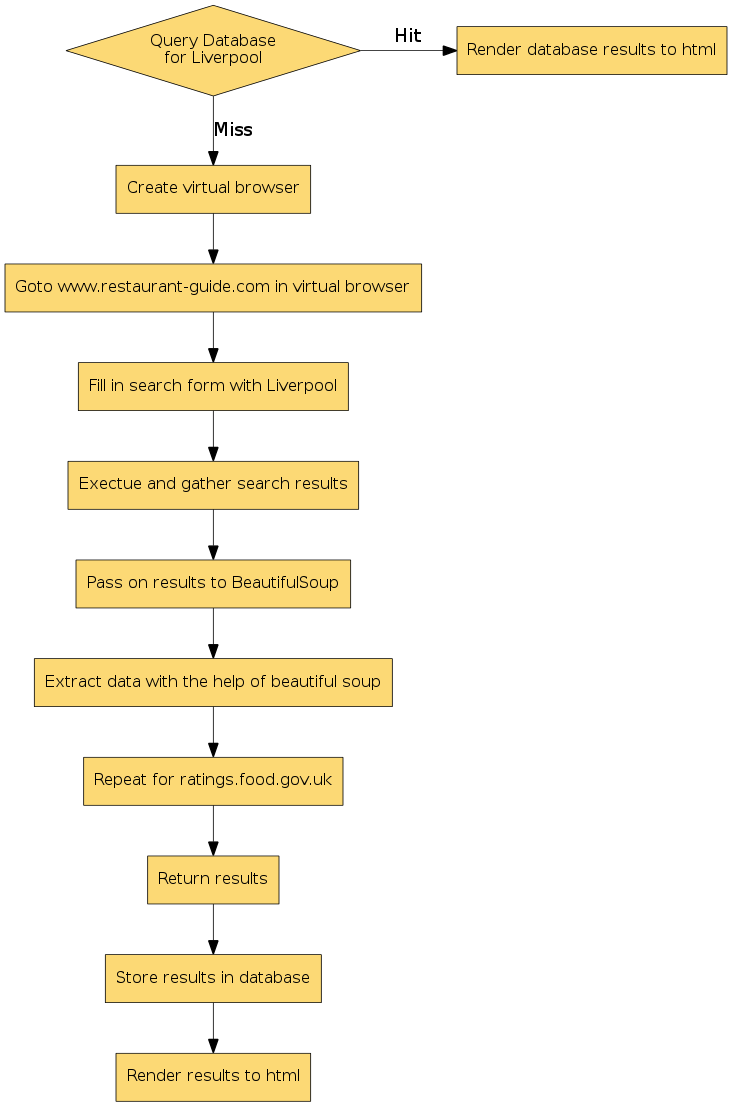
\includegraphics[width=16cm]{fig/flow_chart.png}
\end{figure}


\chapter{Implementation and Testing}
This chapter will highlight the implementation of the mashup and executing it. In general, the working of the mashup works exactly as specified in the scraping program described in Chapter 3. In the next section, we will test the application and assess its working on different search queries.

\section{Implementation}
The complete mashup system comprises of two Python programmes which form the core working components of the mashup. Additionally, the HTML file templates form the structure of the user interface, the results page, a JavaScript and CSS file. All the source code for the project is available in the appendices. In order to execute the mashup, the main.py file has to be compiled. We tested this on a computer with Windows 7.  Windows Powershell or the cmd prompt can be used. Additionally, this was also tested in a Linux environment.

The implementation is relatively straightforward. All the source code files are in a folder called restaurantGO. The program is a local server where the pc’s ip address and its port are initialized in main.py file. Once main.py is executed, the user interface page is opened in the web browser. The mashup is basically designed to accept cuisine name as the user query and it displays the restaurants of that cuisine with predefined categories as specified in the working of the mashup. Hence, the mashup can only display results of restaurant information taken from the restaurant-guide.com which was used for mashing the data.

\section{Testing}

In this section, we execute the mashup using cuisine queries and explain about the details obtained.

Upon executing the mashup with the cuisine query as 'British', one of the obtained results looks as follows(normally, a list of restaurants is obtained and structured).

\begin{figure}[!htb]
  \centering
  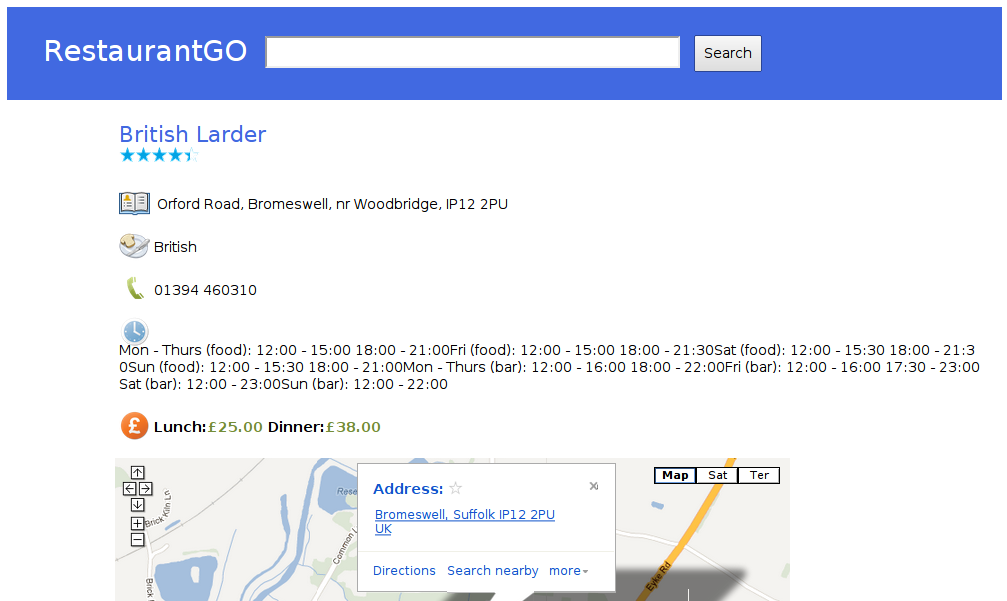
\includegraphics[width=16cm]{fig/restaurant_go_results_british.png}
  \caption[ RestaurantGo search results for  British cuisine]
  {shows search results for British cuisine}
\end{figure}


The above query displays a list of 10 or more restaurants of British cuisine. There also exists an option to choose more results. There are some loading delays which can be attributed to Google maps locations being displayed, which may take a while to load.
The mashups works well with providing a cuisine name as a search query. Similarly, the results for 'Chinese' as the query, are shown in Figure ~\ref{fig:4.2}.

\begin{figure}[!htb]
  \centering
  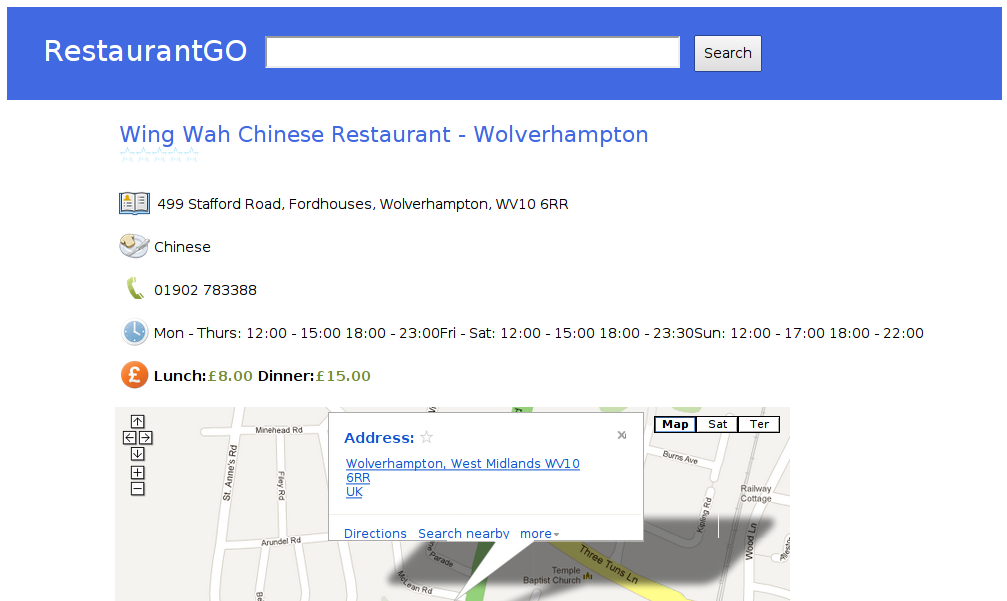
\includegraphics[width=16cm]{fig/restaurant_go_results_chinese.png}
  \caption[ RestaurantGo search results for Chinese cuisine]
  {shows search results for Chinese cuisine}
  \label{fig:4.2}
\end{figure}


With these results, it can be asserted that the mashup works well with cuisine names as queries from the user to get the necessary details of a restaurant's record, such as its address and a Google maps location display for easy navigation. It’s also useful to display the opening and closing times so that the users can plan their schedule and be organized so as to visit the restaurant at their convenience. Budget minded users can check out the prices of the restaurant before making their decision to visit the restaurant.

Moreover, more complex queries, such as 'Italian Coventry' or 'Coventry Italian'(the order does not matter) can also be done, to filter out results for a specific desired location.

Although the mashup works for the cuisines and locations, as in the test case, we did also try it out with some random gibberish text or even normal phrases like “welcome”, “hello” etc. and it produced an error page.
As far as testing of the mashup goes, it works only with cuisine names that are well versed with the restaurant-guide.com website.

\section{Evaluation}
Apart from testing the system, a survey was conducted allowing users to perform an evaluation of the system. Evaluations were recorded based on SUS (System Usability Scale) questionnaire \cite{20} in terms of efficiency, effectiveness and satisfaction. The group of users mainly comes from computer science background. The evaluations are as follows:

\subsection{User 1}
\textbf{Regarding search:}

\begin{itemize}

\item \textbf{Effectiveness} (can users successfully achieve their objectives): I think users can, because the search results cover many types of cuisines, I got numerous results when searched for British, Italian, Indian, Pakistani, African, etc - so all types of keywords get matched. The maps show up each place with postcode, so it helps to straightaway take this info, also quite some important details like opening times, price, phone no, etc. However scope for improvement is that results are mostly in London or Edinburgh, Manchester, Liverpool, etc.. It would help if results are matched based on distance, so I would be more likely to use this system.
\item \textbf{Efficiency} efficiency is pretty fast, and there is hardly any delay, so this is taken care of.
\item \textbf{Satisfaction} (was the experience satisfactory): Apart from the fact that results are ignorant of distance from current location, the search results and the details given are pretty satisfactory. User will be pretty likely of using this system.
  
\end{itemize}

\subsection{User 2}

\begin{itemize}
  
\item \textbf{Effectiveness} The search is quick and efficient. It is able to find all data containing the search tag and displays it in a neat manner.

\item \textbf{Efficiency} It is a quick system and there is little lag between placing a search query and getting results, however since the results are not filtered finding the exact result might be more time consuming.

\item \textbf{Satisfaction} Yes I would say that the experience was satisfactory. 
\item \textbf{Note} I have noticed that your code breaks on unknown search queries, I would recommend you put in some error handing that breaks gracefully and serves up an error message of some sort. Its never nice for a program to break in the back with no indication in the front.

\end{itemize}

\subsection{User 3}

\begin{itemize}
\item \textbf{Effectiveness} (can users successfully achieve their objectives):
        Users are presented with a list of restaurants upon submitting a choice of cuisine. It would be great if the user is given some feedback as to how the results are sorted and/or if the sorting order could be changed on Price or Location (Distance).

\item \textbf{Efficiency} (how much effort and resource is expended in achieving those objectives):
        Results are easily obtained by simply typing in your choice. The results are fetched and presented quickly.

\item \textbf{Satisfaction} (was the experience satisfactory):
        For a single cuisine search, the results were excellent.

\item \textbf{Scope} It might be worthwhile for a future version to offer more than one choices of cuisine to search upon even though the data-source only offers one cuisine type. Additionally, AND and OR logic could be incorporated to support more complex queries.

\end{itemize}

\subsection{User 4}

\begin{itemize}
\item \textbf{Effectiveness} Depends on what the user is searching for , it gives satisfying results when we search with keywords such as cuisine name and  name of the city. But it leaves the user wanting more features such as intelligent searching.

\item \textbf{Efficiency} The application is pretty efficient when it comes to searching with the help of keywords. The results in most of the cases were correct.

\item \textbf{Satisfaction} Much work still needs to go in the application so that it becomes as an application which can be used by a larger amount of people. But on knowing the keywords, the search was pretty efficient and satisfactory.
\end{itemize}

\subsection{User 5}

\begin{itemize}
\item \textbf{Effectiveness} It is clear and easy to use. But I try to enter something like Burmese, it does not seem to like it. Some words seem to work fine, when I run second time.

\item \textbf{Efficiency} It can show the results very quickly actually. Is the result based
on my geographical location?

\item \textbf{Satisfaction} Yes. It would be nice to have something like you are this much away
from this restaurant, or your local alternatives are these.
\end{itemize}

The application was tested by five users and their evaluations were recorded. Overall, users were satisfied with the experience. They did point out some visual formatting issues and lack of an error page for exceptional query searches. For instance,the application doesn't work on non-cuisine names and random text, so this was fixed by providing an output message "search found 0 results". A problem specified by majority of the users that the results are drawn at random and are not based on user's geographical distance. Conducting a test with 5 users was quite advantageous since a common usability problem was detected \cite{27}.
\chapter{Results and Discussion}

This chapter gives an overview of the results obtained and whether these were achieved within the scope of our project and how satisfactory these results are with respect to the objectives and aims of the project. Then, we discuss the importance of these results; explore the limitations faced during the development and the difficulties encountered.

\section{Results}

Upon conceiving the objectives of this project, it is safe to iterate that these objectives were achieved. Our project involved designing a semantic mashup which can gather required data from several source websites and mash the results obtained into our site. The obtained results were also categorized via semantic tags, which were the basic parameters defining any restaurant. As mentioned in the previous chapter, the mashup was also tested with various cuisines and locations, and the results were satisfactory in terms of providing detailed information of restaurants based on our own categorizations.

The results were obtained as we have ascertained based on the working of the mashup. They were some loading time issues which were mainly due to the Google map locations being displayed for each restaurant result. Apart from this, the mashup worked fine with a wide variety of cuisine name queries. Since the user will be aware of what search results will be obtained for cuisine search, testing it with some random terms apart from cuisine names gave us a typical error message pertaining to an attribute error. While developing the mashup, we didn’t take into account the usage of search terms apart from cuisine and location names. For such erroneous queries, we can provide an exception result, such as a customized error message, which can be produced upon searching a non-existent name. The message generated can ask the user to search for a cuisine or location name, since the mashup is mainly programmed for that purpose and can take the user back to the home page.

In terms of the user experience, the results produced can be quite useful for a user in search of a restaurant. Semantic mashups differ from other mashups in terms of providing metadata to the data to make sense of that information. Using the restaurant websites directly, it may be difficult to look for the required information for a restaurant. By placing custom designed columns, each restaurant’s data gathered was filtered only to provide the relevant ones. In our case, we took some attributes like its address, opening times and prices. These attributes are crucial for a user to make a decision so as to visit the restaurant or not. In this way, this semantic mashup does provide a service of recommending restaurants to users based on this collated data. Moreover, the interface is simple but self-explanatory, because all users are used to querying in a search engine, and the program doesn't require more input than that.

\section{Limitations and difficulties}
In terms of limitations, we considered potentially using some of the APIs for restaurant websites. But API reliability was a common problem for some sites and when it’s not up to date, it would cause problems in gathering the required data. Some of the APIs would not be documented properly and most of them would require the mashup developer to have knowledge at an advanced level.

Initially, our plan in the thesis was to have total control of the semantic mashup by programming it completely and scraping off the relevant data automatically. It was never the project’s intended goal to use an API to gather the data, but nevertheless, it was researched upon. However, we were able to gather ratings of the restaurants from a different source by utilizing the website’s API. The results were quite satisfactory. As specified in chapter 2, we also researched many of the software tools that can help to  create mashups without the need of any programming. They weren’t used in the project, since the functionality is pretty limited and couldn’t help in accomplishing our project goals, which have more emphasis in data scraping.

Some of the difficulties encountered were mainly programming issues and choosing the programming language itself. Python was chosen since it was simple and flexible. Python also had useful libraries that make it suitable for web programming. We did encounter difficulties due to some data formats that were unstructured.

\chapter{Conclusion}
We will conclude this thesis with some suggestions for future work and a summary of the work done.

\section{Future work}
The semantic mashup was indeed successful in extracting data from the source and the output was displayed with semantic annotations. This can be further extended to add newer features. For instance, it would be useful to add images of the restaurants along each result so that the user will have a view of its environment. It will be quite difficult, since images of these particular restaurants will be scattered across web pages, and there won’t be a single source or format available, but multiple ones. Google images API has been deprecated, but its custom search API, which also supports images can be looked into regarding this.

Since the mashup was able to scrape data off a single source, we can include another restaurant website as well using the same methodology. The other restaurant websites could support other useful features. For instance, there were some websites that can support booking a table at a restaurant and this feature can be implemented in order for the user to make reservations.

Using Web 2.0 tools, Facebook or other social networks API can be implemented. Users can log in and share recommendations with others. Reviews can be added and shared as well.

There were some delays in processing the pages due to Google maps causing load delays. Although we didn’t use Google maps API, its API can be studied and utilized in order to provide a better service of displaying locations of the restaurant. Possible integration can also specify a route via GPS from the user’s location to the restaurant. This can be looked into and it maybe well worth the effort.



\section{Conclusion}
We developed a simple and basic semantic mashup which extracts the relevant data and provides the output in a semantically enhanced way. We were also able to obtain the results needed akin to our project goals. We did have some difficulties in programming the mashup and using the necessary libraries, but it was a good learning experience in the context of this research project. Moreover, the mashup is extensible and several features specified in the previous section can be implemented to enhance the user experience.

Overall, our work demonstrates using Web 2.0 technology(such as mashups) as well as Semantic Web methods(such as annotation and metadata), and extracting the synergetic effects of these two different directions working together.




\cleardoublepage
\phantomsection
\addcontentsline{toc}{chapter}{Bibliography}
\bibliographystyle{IEEEtranN}
\begin{thebibliography}{27}

\bibitem{1} Benjamin Erb , Jan-Patrick Elsholz and Franz J. Hauck \emph{``Semantic Mashup: Mashing up the information in Today's World Wide Web - An Overview''}, Technical Report Document Number: VS-R08-2009  Institute for Distributed Systems, University of Ulm, 2009

\bibitem{2} Mashup, http://en.wikipedia.org/wiki/Mashup\_(web\_application\_hybrid)

\bibitem{3} Future Generation Communication and Networking Symposia, International Conference on, Vol. 2 (2008), pp. 50-53, doi:10.1109/FGCNS.2008.73

\bibitem{4} D. Merill \emph{``Mashups: the new breed of web app''}, IBM Web Architecture Technical Library (2006)

\bibitem{5} mechanize, http://wwwsearch.sourceforge.net/mechanize/

\bibitem{6} Beautiful Soup, http://www.crummy.com/software/BeautifulSoup/bs4/doc/

\bibitem{7} In IUI '08: Proceedings of the 13th international conference on Intelligent user interfaces (2008), pp. 139-148, doi:10.1145/1378773.1378792

\bibitem{8} Nan Zang, Mary R. Bosson, Vincent Nasser. \emph{``Mashups: who? what? why?''} In CHI '08 extended abstracts on Human factors in computing systems (2008), pp. 3171-3176, doi:10.1145/1358628.1358826

\bibitem{9} Focused crawler, http://en.wikipedia.org/wiki/Focused\_crawler

\bibitem{10} isbnnetinclj (to find online prices of books in india), https://github.com/swaroopch/isbnnetinclj

\bibitem{11} Jin Yu, Boualem Bentallah, Fabio Casati, Florian Daniel. \emph{``Understanding mashup development''} IEEE Internet Computing In Internet Computing, IEEE, Vol. 12, No. 5. (09 September 2008), pp. 44-52, doi:10.1109/MIC.2008.114

\bibitem{12} Alfredo Alba, Varun Bhagwan, Tyrone Grandison. \emph{''Accessing the deep Web''} Commun. ACM, Vol. 50, No. 5. (May 2007), pp. 94-101, doi:10.1145/1230819.1241670

 \bibitem{13} R. J. Ennals \& M. N. Garofalakis (2007). \emph{``MashMaker: mashups for the masses''}. In SIGMOD'07: Proceedings of the 2007 ACM SIGMOD international conference on Management of data,pp. 1116-1118, New York, NY, USA. ACM..

\bibitem{14} R. Tuchinda, et al. (2008). \emph{``Building Mashups by example''}. In IUI '08: Proceedings of the
  13th international conference on Intelligent user interfaces, pp. 139-148, New York, NY, USA.
  ACM.

\bibitem{15} Klocker,Christoph. \emph{``Mashups : A new concept in web application programming''}. Saarbrucken:VDM Verlag Dr.Muller,2008.

\bibitem{16} N. Kulathuramaiyer (2007). \emph{``Mashups: Emerging Application Development Paradigm for a Digital Journal''}. Journal of Universal Computer Science 13(4).

\bibitem{17} R. Floyd, et al. (2007). \emph{``Web Mash-ups and Patchwork Prototyping: User-driven technological innovation with Web 2.0 and Open Source Software''}. In HICSS '07: Proceedings  of the 40th Annual Hawaii International Conference on System Sciences, Washington, DC, USA. IEEE Computer Society.

\bibitem{18} Hye-Jin Jin; Hong-Chul Lee; , \emph{``Web services development methodology using the mashup  technology''}, Smart Manufacturing Application, 2008. ICSMA 2008. International Conference on, vol., no., pp.559-562, 9-11 April 2008.

\bibitem{19} Nan Zang, \emph{``Mashups for the web-active user''}, vlhcc, pp.276-277, 2008 IEEE Symposium onVisual Languages and Human-Centric Computing, 2008.

\bibitem{20} System Usability Scale. http://en.wikipedia.org/wiki/System_usability_scale

\bibitem{21} ICN '07 Proceedings of the Sixth International Conference on Networking
  Page 32

\bibitem{22} Wong, Jeffrey and Hong, Jason I., \emph{``Making Mashups with Marmite: Towards End-User Programming for the Web''} (2007). Human-Computer Interaction Institute. Paper 65.
  http://repository.cmu.edu/hcii/65

\bibitem{23} Programmable Web. http://www.programmableweb.com/

\bibitem{24} Flask. http://flask.pocoo.org/

\bibitem{25} Yahoo pipes. http://pipes.yahoo.com/pipes/

\bibitem{26} Microsoft popfly. http://www.popfly.ms/microsoft-popfly/

\bibitem{27} Usability testing with 5 users. http://www.useit.com/alertbox/20000319.html

\end{thebibliography}


\lstset{
  %  basicstyle=\footnotesize,
  frame=tb,
  numbers=left,
  numberstyle=\color{black},
  stepnumber=1,
  numbersep=5pt,
  backgroundcolor=\color{white},
  showspaces=false,
  showstringspaces=false,
  showtabs=false,
  rulecolor=\color{black},
  tabsize=2,
  captionpos=b,
  breaklines=true,
  breakatwhitespace=false,
%  title=\lstname,
  keywordstyle=\color{red},
  commentstyle=\color{gray},
  stringstyle=\color{ForestGreen},
  escapeinside={\%*}{*)},
  morekeywords={*,...},
  identifierstyle=\color{blue}
}

\appendix
\chapter{Software used}

The programs were written in Notepad++ and can be run on a compatible web browser. We would recommend Google chrome. The python version used is 2.7.2 which is freely available from the official python website supported by the Python software foundation.

A few python libraries Beautiful Soup and mechanize are used. Their documentations can be accessed in [6] and [5] respectively.

A read me file has been included with further instructions in installing the necessary software for the python files to execute successfully.

\chapter{Code Listing -- main.py}
\lstinputlisting[language=Python]{../main.py}

\chapter{Code Listing -- restaurant\_sites.py}
\lstinputlisting[language=Python]{../restaurant_sites.py}


\end{document}
